% Pilot report: Investigate, Fix or Escalate.
% LaTeX version of documentation/pilot_report.md (10 November 2026).
% Figures are read from results/pilot/figures/.
% Build: ..\..\tools\tectonic.exe pilot_report.tex   (or run build.bat)

\documentclass[11pt,a4paper]{article}

\usepackage[T1]{fontenc}
\usepackage{lmodern}
\usepackage[a4paper,left=2.2cm,right=2.2cm,top=2.2cm,bottom=2.4cm]{geometry}
\usepackage{amsmath}
\usepackage{graphicx}
\usepackage{enumitem}
\usepackage{booktabs}
\usepackage{tabularx}
\usepackage{array}
\usepackage{float}
\usepackage{caption}
\usepackage{xcolor}
\usepackage{microtype}
\usepackage{fancyhdr}
\usepackage[hidelinks]{hyperref}

\graphicspath{{../../results/pilot/figures/}}

\setlength{\parindent}{0pt}
\setlength{\parskip}{5pt}
\setlist{leftmargin=1.5em, itemsep=2pt, topsep=2pt}
\captionsetup{font=small, labelfont=bf}
\newcolumntype{L}{>{\raggedright\arraybackslash}X}
\newcolumntype{R}{>{\raggedleft\arraybackslash}X}
\renewcommand{\arraystretch}{1.15}
\newcommand{\file}[1]{\texttt{\small #1}}

\pagestyle{fancy}
\fancyhf{}
\lhead{\small Pilot Report}
\rhead{\small Opol Charis}
\cfoot{\small \thepage}
\renewcommand{\headrulewidth}{0.4pt}

\begin{document}

% ---------------------------------------------------------------- title
\begin{center}
\IfFileExists{../../research/proposal/UCU-Logo.png}{
\includegraphics[height=1.6cm]{../../research/proposal/UCU-Logo.png}\par\vspace{4pt}}{}
{\bfseries Uganda Christian University\\
Faculty of Engineering, Design and Technology\\
Department of Computing and Technology}\par\vspace{10pt}
{\LARGE\bfseries Pilot Report}\par\vspace{4pt}
{\large Investigate, Fix or Escalate: A Rule-Constrained Reinforcement Learning Agent for IT Incident Triage under Ambiguous Evidence}\par\vspace{8pt}
Opol Charis \quad Reg.\ No.\ S24B23/003 \quad B29654\\
10 November 2026
\end{center}

\vspace{4pt}
\noindent\fcolorbox{black!40}{black!4}{\parbox{\dimexpr\linewidth-2\fboxsep-2\fboxrule}{\small
\textbf{Status: pilot.} The scenario model comes from one developer of the Directorate (Part~1 and Part~2 workbooks), not from the planned Directorate elicitation, and several settings are the researcher's. The results show that the method runs, learns and can be evaluated as Chapter~3 plans. They are not thesis findings.\\[3pt]
\textbf{Detail:} the step-by-step record is \file{documentation/pilot\_experiment\_plan.md} (Phases 0 to 9) and \file{documentation/phase9\_log.md}. Tables: \file{results/pilot/comparison.md}, \file{results/pilot/phase5.md}, \file{results/pilot/prototype\_v3.md}.}}

% ---------------------------------------------------------------- 1
\section{Summary}

\begin{enumerate}
  \item \textbf{The full pipeline works}: scenario model, simulated environment, safety mechanism, baselines, three learning agents, the evaluation of Chapter~3 Experiments 1 and 2, and a prototype that reads a ticket and its logs, decides, and carries the decision out on a fictional repository.
  \item \textbf{Fix with verification is in place.} A fix is applied and verified. If it fails, the agent pays for the harm, sees that the fix failed and goes on, and after two failed fixes a person takes over. All results in Sections~\ref{sec:training} and~\ref{sec:results} use this setting.
  \item \textbf{The agents match the strongest baseline, but do not beat it.} At the elicited escalation cost, the penalty-only ($-0.24$) and unconstrained ($-0.28$) agents edge past the threshold policy ($-0.38$), and the agent with the safety mechanism is level with it ($-0.41$). The intervals overlap. Every agent is far ahead of the scripted, initial-symptom and always-escalate baselines on return.
  \item \textbf{The safety mechanism does its job, but at a cost the pilot exposes.} It brings executed violations to zero (unconstrained: 7.6\% of incidents). However, the agent behind it keeps proposing rule-breaking fixes (22\% of its proposals, still about 20\% at the end of training), because in the pilot a blocked proposal costs only a step. The penalty-only agent learned to propose none and has the best compliant success.
  \item \textbf{Against the Chapter~3 criteria, H1 and H2 are not supported in this pilot} (Section~\ref{sec:hypotheses}). This is useful: it shows where the design needs attention before the Directorate model, chiefly the cost of a blocked proposal and the strength of the scripted baseline once fixes are verified.
\end{enumerate}

% ---------------------------------------------------------------- 2
\section{What was built}

\begin{table}[H]
\centering\small
\caption{Components of the pilot.}
\begin{tabularx}{\linewidth}{@{}p{2.6cm}Lp{4.2cm}@{}}
\toprule
Part & What it is & Where \\
\midrule
Scenario model v2 & 8 causes, 11 checks (one delegated to a language model, D11), 4 symptoms, 5 rules, with per-cause owner and ``fixed by a code change'' flag. From the pilot developer's Part~1 and Part~2 workbooks & \file{experiments/pilot/ pilot\_model\_v2.json} \\
Environment & Gymnasium environment of Chapter~3; noise, missing checks and overlap controls; optional fix with verification & \file{src/sim/} \\
Safety mechanism & Checks every proposal against the rules; a blocked proposal is returned once, a second block in a row escalates & \file{src/rules/safety.py} \\
Baselines & Always escalate, initial-symptom, scripted checklist, confidence threshold (given the likelihood model) & \file{src/agents/baselines.py} \\
Agents & Masked Double DQN: with the safety mechanism, unconstrained, penalty-only & \file{src/agents/dqn.py} \\
Experiments & Experiments 1 and 2 with the escalation-cost sensitivity analysis & \file{experiments/pilot/ run\_comparison.py}, \file{evaluate\_comparison.py} \\
Prototype & Ticket and logs, then reader, agent, safety mechanism, verification, then a draft pull request, a fix order or a routed escalation & \file{src/prototype/}, \file{dashboard/ prototype\_app.py} \\
\bottomrule
\end{tabularx}
\end{table}

\paragraph{Fix with verification} (\file{pilot\_settings\_v3.json}). Applying the remedy for cause $j$ takes its apply time. If $j$ is the true cause, the symptoms clear and the incident is resolved. If not, the agent pays the apply time plus the remedy's harm, sees a ``fix failed'' flag for $j$, and $j$ can no longer be chosen. After two failed fixes a person takes over at the escalation cost. The mean harm is set so that a wrong fix followed by escalation costs the elicited $5\times$ escalation on average. It is spread across remedies by how hard each is to undo, following the reasons given for the rules: deleting rows weighs 2.0, rolling back a release or killing a transaction 1.5, and a code change by draft pull request 0.5.

% ---------------------------------------------------------------- 3
\section{Settings}

\begin{table}[H]
\centering\small
\caption{Pilot settings and where each value comes from.}
\begin{tabularx}{\linewidth}{@{}p{4.4cm}Lp{3.6cm}@{}}
\toprule
Setting & Value & Source \\
\midrule
Escalation & 120 min (2 h) & Pilot developer \\
Wrong fix & $5\times$ escalation & Pilot developer \\
Correct fix & $+5$ h & Researcher \\
Check cost, Low / Medium / High & 5 / 15 / 30 min & Researcher \\
Remedy apply times, harm weights, 2 failed fixes, step limit 15 & See \file{pilot\_settings\_v3.json} & Researcher (provisional; for a Part~3 workbook) \\
Noise, missing checks, overlap & 0.1, 0, 0 & Researcher \\
Training & Double DQN, $2\times128$ units, 500k steps, exploration to 5\% by 150k, discount 1.0 & Tuned in Phase 4 \\
Penalty-only agent & 10 per rule-breaking action, training only & Researcher \\
Block cost & None beyond the step it uses (Chapter~3 specifies a small penalty) & Pilot deviation, see Section~\ref{sec:limits} \\
Seeds & 0, 1, 2 for each of 15 runs & Decision of 9 Nov 2026 \\
Evaluation & 5,000 incidents, the same for every policy, from seeds never used in training; baselines tuned on 2,000 separate incidents & Chapter~3 \\
\bottomrule
\end{tabularx}
\end{table}

% ---------------------------------------------------------------- 4
\section{Training}\label{sec:training}

Fifteen runs: the three agents at the elicited escalation cost (Experiment~2), and the agent with the safety mechanism retrained at 60 and 240 minutes (sensitivity analysis). With five runs in parallel, one thread each, a run takes about 70 minutes and all fifteen about 3.5 hours. All fifteen finished.

\begin{figure}[H]
\centering
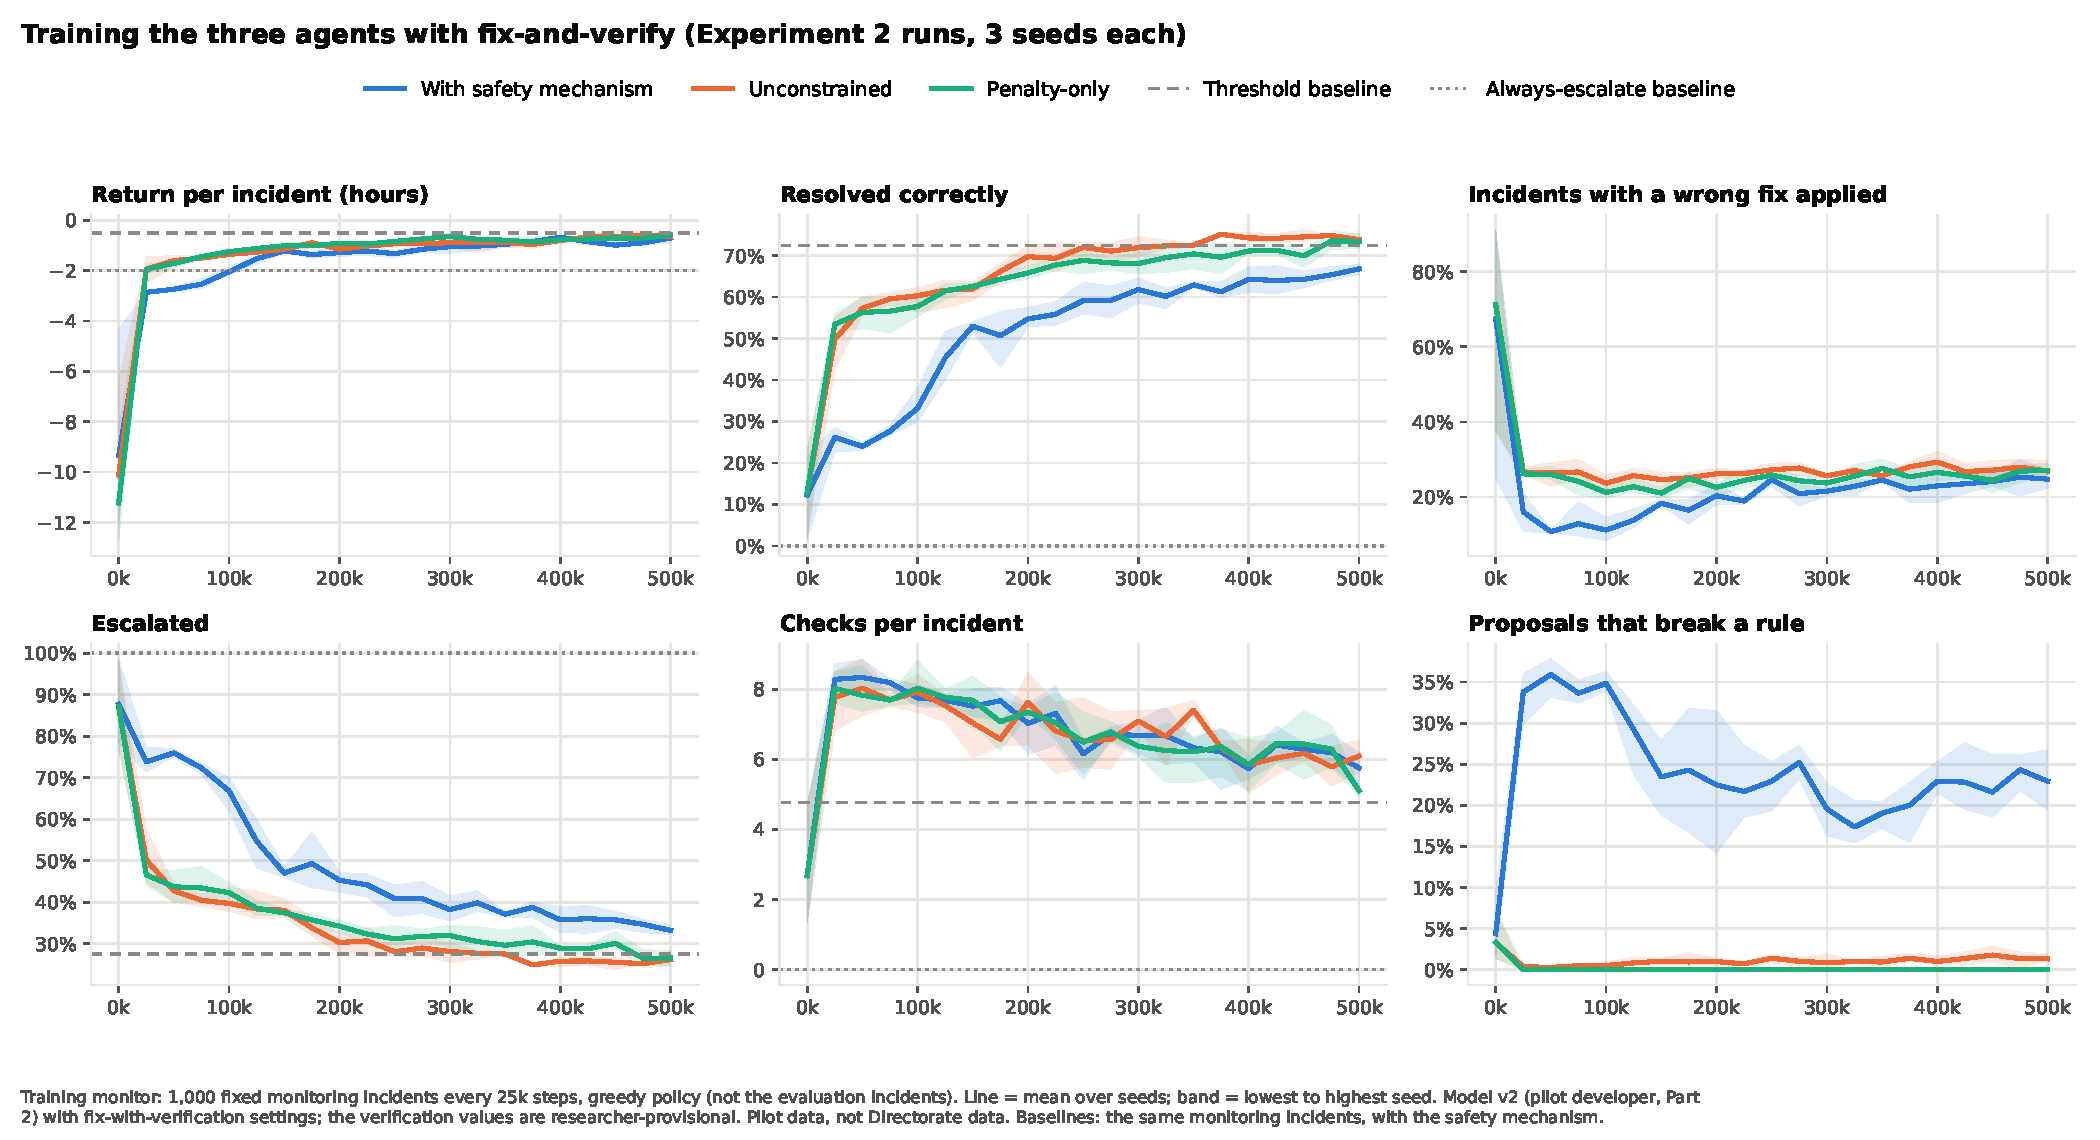
\includegraphics[width=\linewidth]{v3_training_agents.pdf}
\caption{Training the three agents at the elicited escalation cost.}
\label{fig:train-agents}
\end{figure}

\begin{enumerate}
  \item \textbf{All three agents learn.} Return rises from about $-10$ hours (untrained) to between $-0.5$ and $-0.9$ on the monitoring incidents, and every agent passes the always-escalate baseline within 25k steps.
  \item \textbf{The agent with the safety mechanism learns more slowly.} It resolves fewer incidents than the other two for most of training (about 25\% against 55\% at 50k steps) and escalates more. The gap narrows but has not closed at 500k steps.
  \item \textbf{All agents check more than the threshold policy} (5 to 6 checks against 4.7) and are still reducing their checks at the end of training. Longer training may help, as Phase~4 found.
\end{enumerate}

\begin{figure}[H]
\centering
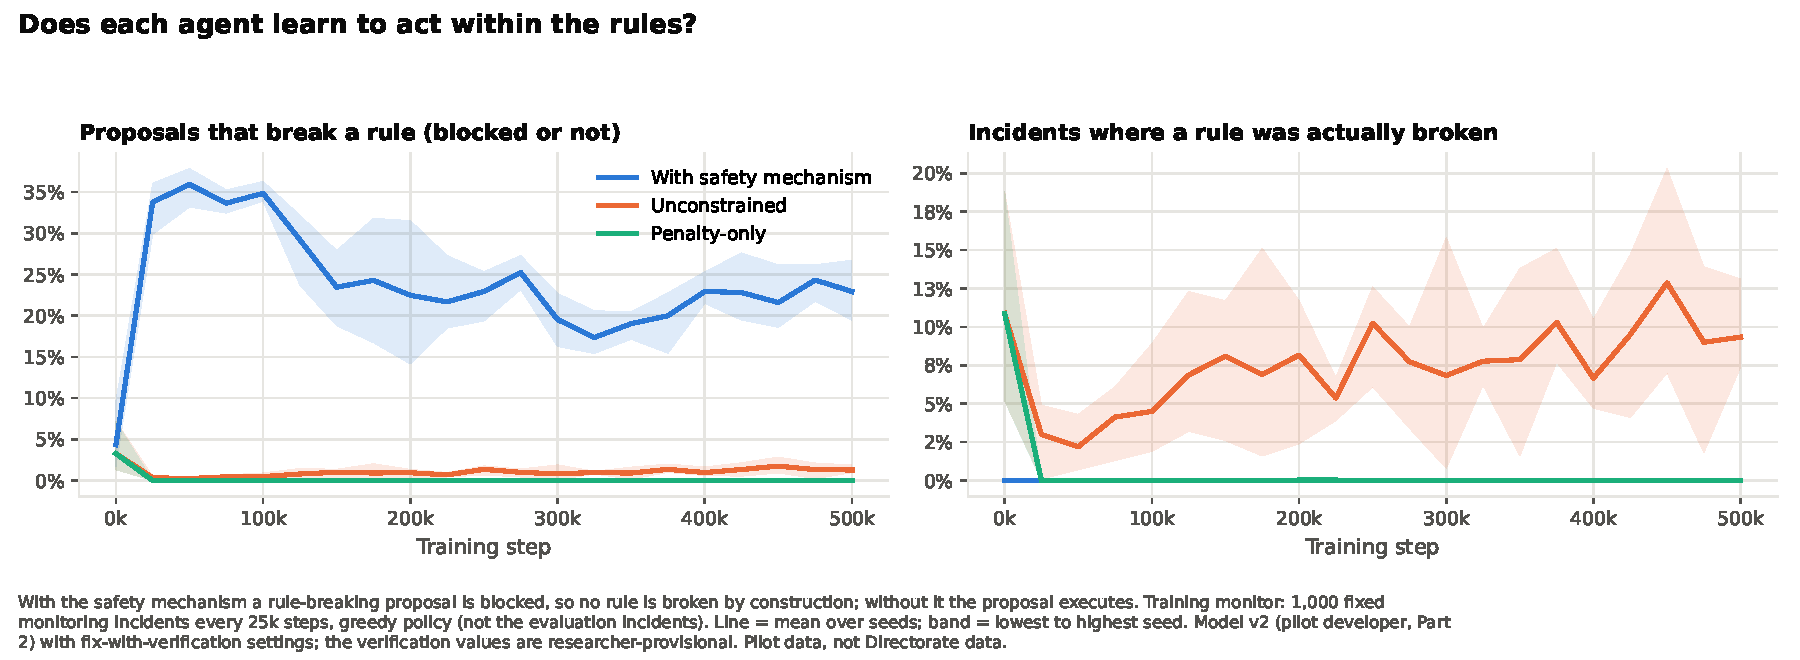
\includegraphics[width=\linewidth]{v3_training_compliance.pdf}
\caption{Rule compliance over training.}
\label{fig:train-compliance}
\end{figure}

\begin{enumerate}[resume]
  \item \textbf{Rule-breaking proposals do not fall far.} With the safety mechanism, they rise to about 35\% early in training and settle around 20 to 25\%. The agent proposes a forbidden fix and lets the mechanism send it back for the required check. The penalty-only agent stops proposing them within 25k steps. The unconstrained agent proposes few (about 1\%), but each one executes, and it breaks a rule in 7 to 13\% of monitoring incidents.
\end{enumerate}

\begin{figure}[H]
\centering
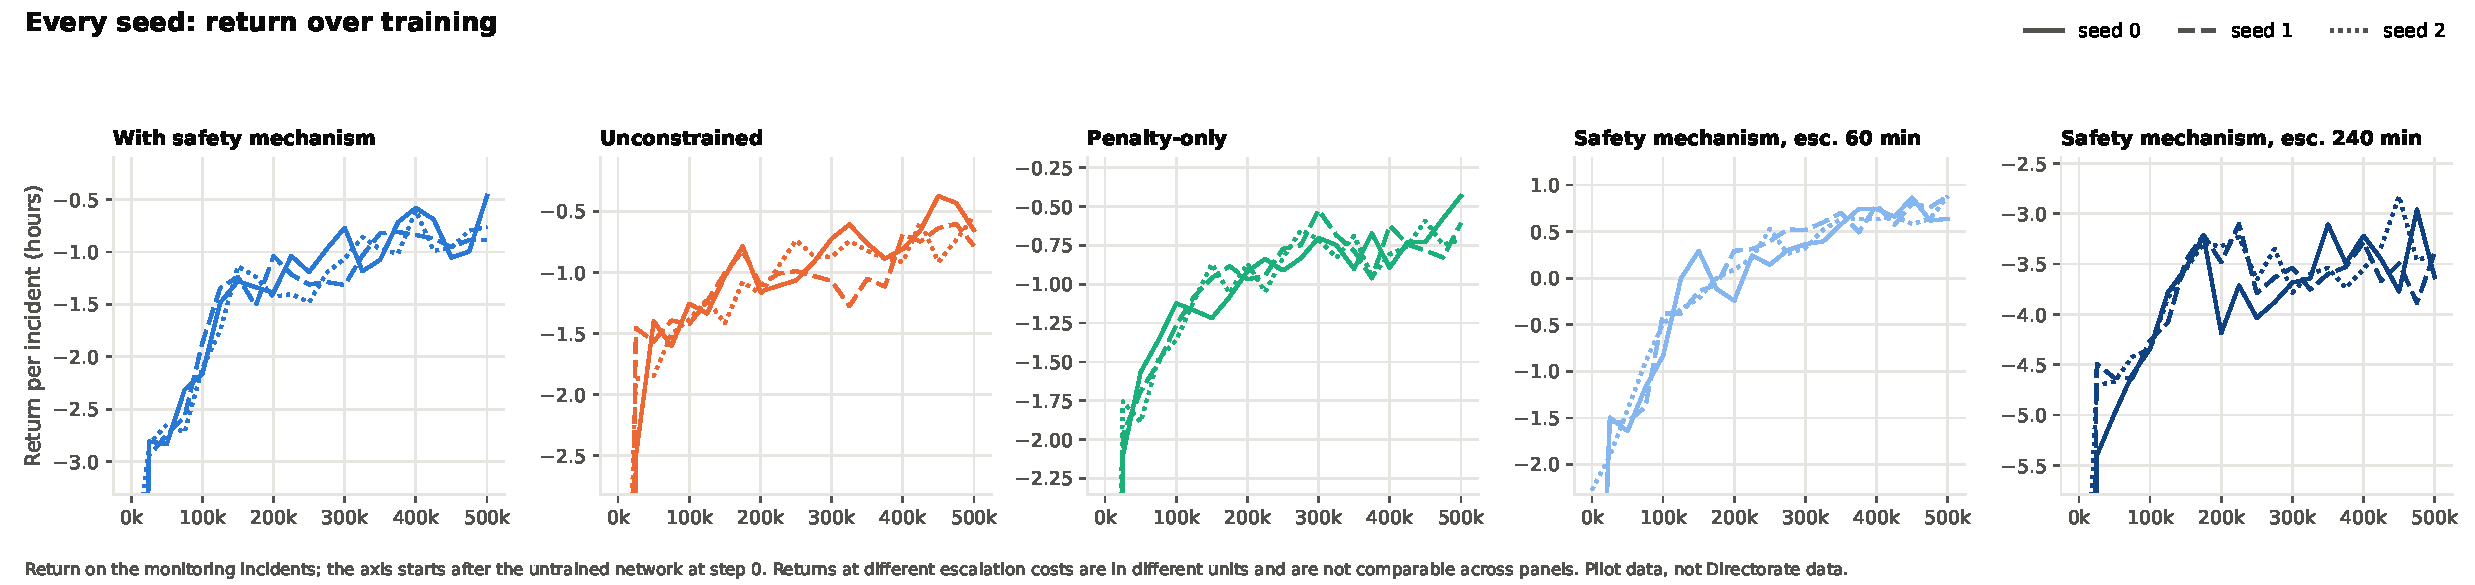
\includegraphics[width=\linewidth]{v3_training_seeds.pdf}
\caption{Every seed of every run.}
\label{fig:train-seeds}
\end{figure}

\begin{enumerate}[resume]
  \item \textbf{Seeds agree closely} at 120 and 60 minutes. At 240 minutes, seed 0 ends about 0.25~h below the other two.
\end{enumerate}

% ---------------------------------------------------------------- 5
\section{Results: Experiments 1 and 2}\label{sec:results}

\begin{figure}[H]
\centering
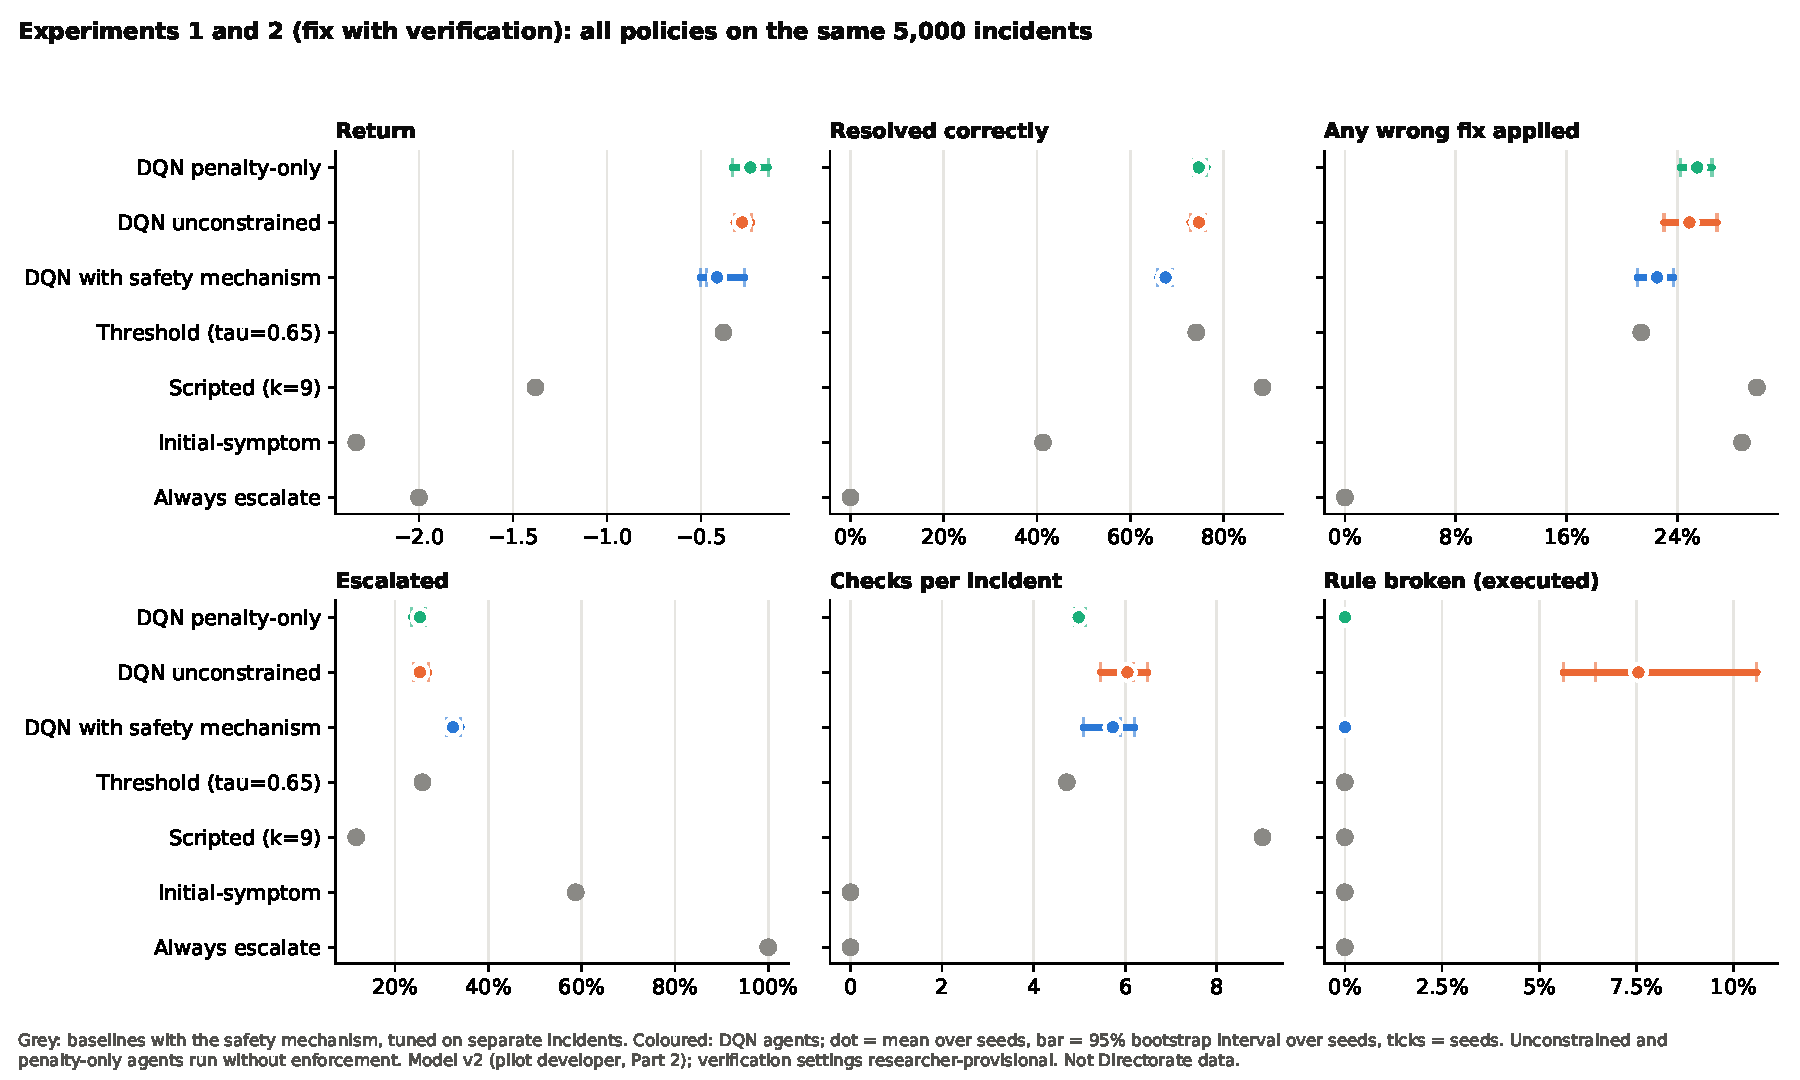
\includegraphics[width=\linewidth]{comparison_policies.pdf}
\caption{All policies on the same 5,000 evaluation incidents.}
\label{fig:policies}
\end{figure}

\begin{table}[H]
\centering\footnotesize
\setlength{\tabcolsep}{3.5pt}
\caption{Experiments 1 and 2 at the base level (escalation 120 min, noise 0.1, no missing checks). Returns in hours; agents are the mean over three seeds with the 95\% interval over seeds.}
\label{tab:main}
\resizebox{\linewidth}{!}{%
\begin{tabular}{@{}lccccccccc@{}}
\toprule
Policy & \shortstack{Return\\(h)} & \shortstack{95\% CI\\over seeds} & Resolved & \shortstack{Any\\wrong fix} & Escalated & Checks & \shortstack{Rule-breaking\\proposals} & \shortstack{Rule broken\\(executed)} & \shortstack{Compliant\\success} \\
\midrule
Always escalate & $-2.00$ & & 0\% & 0\% & 100\% & 0.0 & 0\% & 0\% & 0\% \\
Initial-symptom & $-2.33$ & & 41.3\% & 28.6\% & 58.7\% & 0.0 & 54.7\% & 0\% & 41.3\% \\
Scripted (9 checks) & $-1.38$ & & 88.3\% & 29.7\% & 11.7\% & 9.0 & 0\% & 0\% & 88.3\% \\
Threshold (0.65) & $-0.38$ & & 74.1\% & 21.4\% & 25.9\% & 4.7 & 4.7\% & 0\% & 74.1\% \\
\midrule
DQN with safety mechanism & $-0.41$ & {\scriptsize$[-0.50, -0.27]$} & 67.6\% & 22.5\% & 32.4\% & 5.7 & 22.4\% & \textbf{0\%} & 67.6\% \\
DQN unconstrained & $-0.28$ & {\scriptsize$[-0.32, -0.23]$} & 74.7\% & 24.9\% & 25.3\% & 6.0 & 1.1\% & \textbf{7.6\%} & 67.9\% \\
DQN penalty-only & $-0.24$ & {\scriptsize$[-0.33, -0.14]$} & 74.7\% & 25.4\% & 25.3\% & 5.0 & 0\% & 0\% & 74.7\% \\
\bottomrule
\end{tabular}}
\end{table}

\begin{table}[H]
\centering\small
\caption{Paired comparison with the threshold policy: difference in return (h) on the same incidents, per seed, with the 95\% bootstrap interval over incidents. Positive means the agent did better.}
\label{tab:paired}
\begin{tabular}{@{}lccc@{}}
\toprule
Agent & Seed 0 & Seed 1 & Seed 2 \\
\midrule
With safety mechanism & $+0.11$ $[-0.02, +0.24]$ & $-0.12$ $[-0.28, +0.02]$ & $-0.09$ $[-0.24, +0.06]$ \\
Unconstrained & $+0.09$ $[-0.05, +0.22]$ & $+0.06$ $[-0.08, +0.19]$ & $+0.15$ $[+0.02, +0.28]$ \\
Penalty-only & $+0.14$ $[+0.01, +0.28]$ & $+0.24$ $[+0.09, +0.39]$ & $+0.05$ $[-0.09, +0.18]$ \\
\bottomrule
\end{tabular}
\end{table}

\begin{figure}[H]
\centering
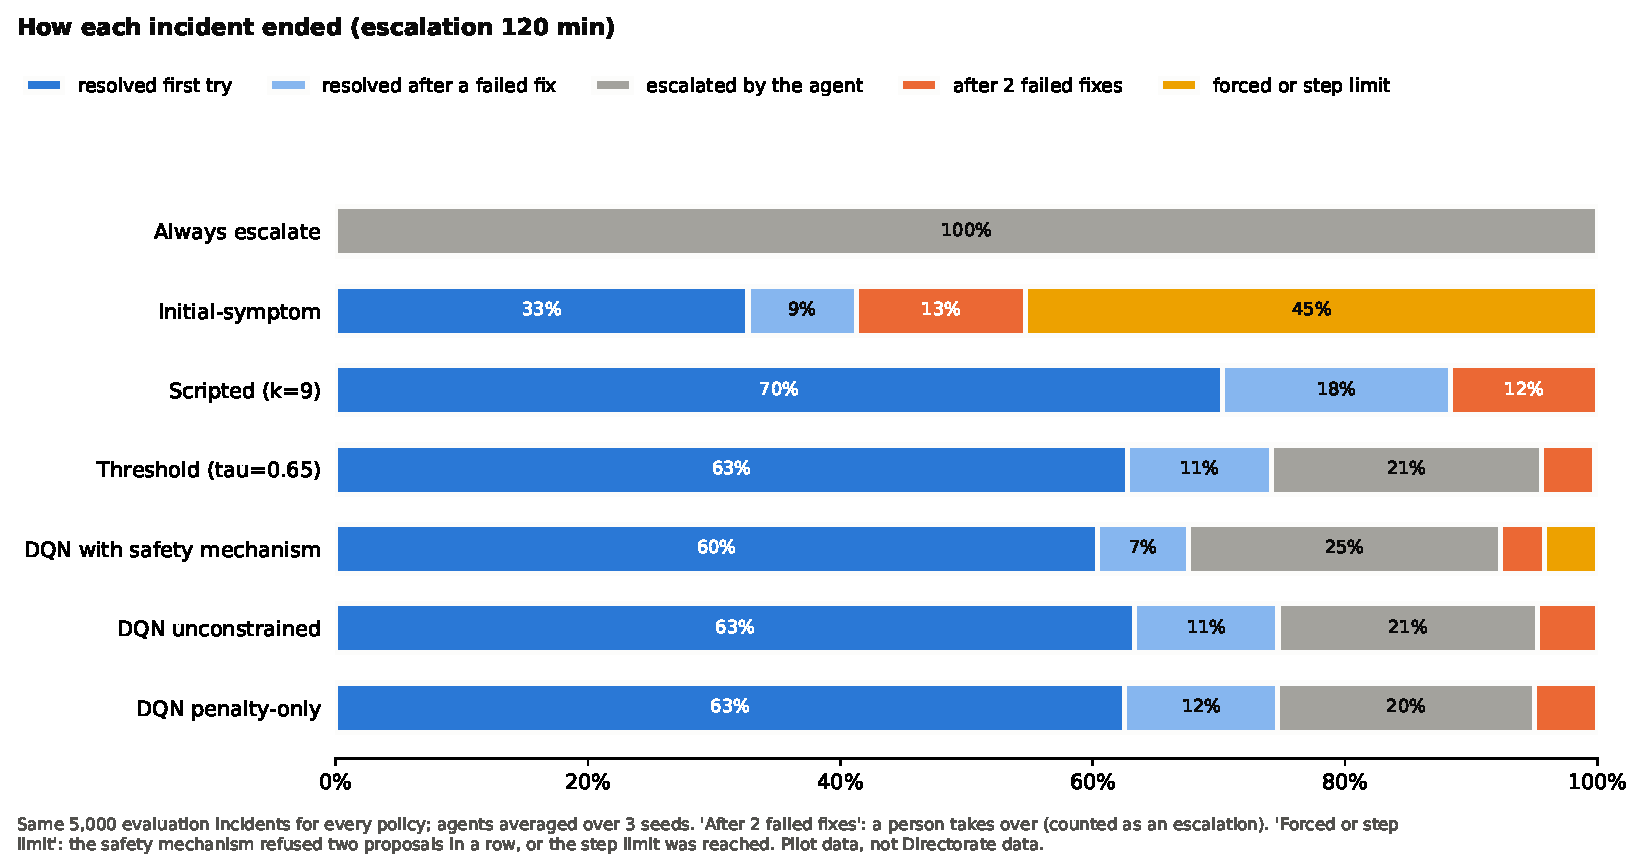
\includegraphics[width=\linewidth]{comparison_outcomes.pdf}
\caption{How each incident ended, by policy.}
\label{fig:outcomes}
\end{figure}

\begin{enumerate}
  \item \textbf{The learned agents reach the threshold policy.} That policy is given the likelihood model the agents must learn, so Chapter~3 does not expect them to beat it. Two of three penalty-only seeds and one unconstrained seed do so with intervals above zero (Table~\ref{tab:paired}). The agent with the safety mechanism is level with it.
  \item \textbf{The scripted checklist resolves the most incidents but has a poor return.} With verification, a checklist that always runs nine checks and then tries the most probable fix, and then the next one, resolves 88\% of incidents. It pays for this with nine checks every time and a wrong fix in 30\% of incidents. The comparison on resolution alone therefore favours it (see H1 in Section~\ref{sec:hypotheses}).
  \item \textbf{The agents use verification sparingly.} They resolve 7 to 12\% of incidents after a failed fix, against 18\% for the scripted checklist. They escalate the rest themselves (20 to 25\%) rather than run into the two-fix limit (3 to 5\%).
  \item \textbf{The safety mechanism adds forced escalations.} 4\% of its incidents end because two proposals in a row were blocked or the step limit was reached. No other learned agent has any.
  \item \textbf{Escalation quality is the same for every learned agent} (MCC 0.54 to 0.55, threshold 0.57). Escalating an incident is what the reference label expects about as often as it is for the threshold policy.
\end{enumerate}

\subsection{Sensitivity to the cost of escalation}

The agent with the safety mechanism was retrained with escalation at 60 and 240 minutes, and the threshold and scripted baselines were re-tuned at each cost. A wrong fix stays at $5\times$ escalation, so its harm scales too, while the reward for a correct fix stays at 5 hours. ``Escalation 240 min'' therefore also makes every mistake relatively costlier.

\begin{figure}[H]
\centering
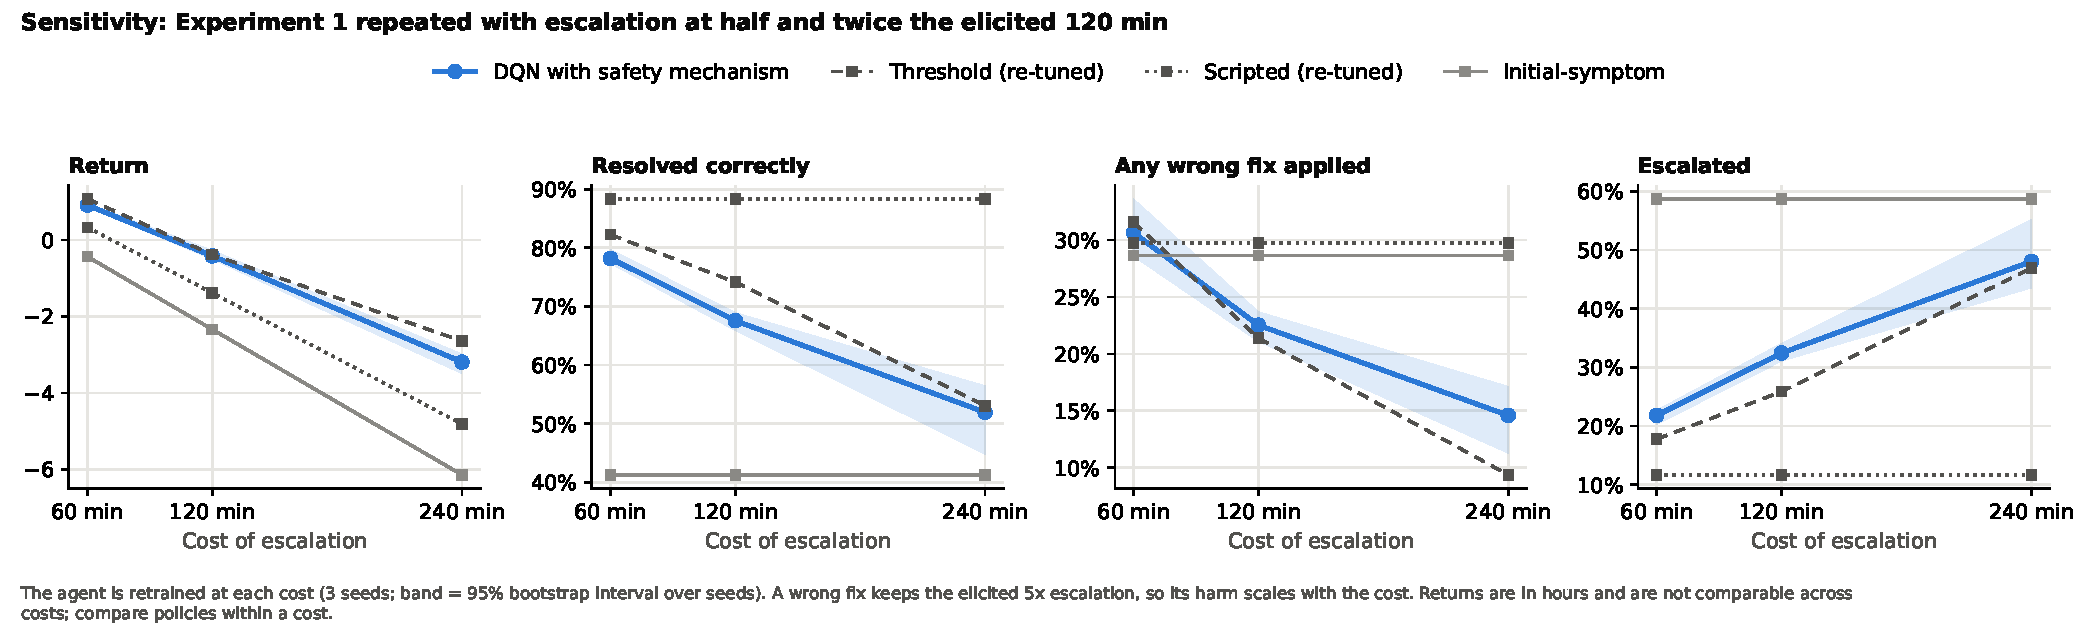
\includegraphics[width=\linewidth]{comparison_sensitivity.pdf}
\caption{Sensitivity to the cost of escalation.}
\label{fig:sensitivity}
\end{figure}

\begin{figure}[H]
\centering
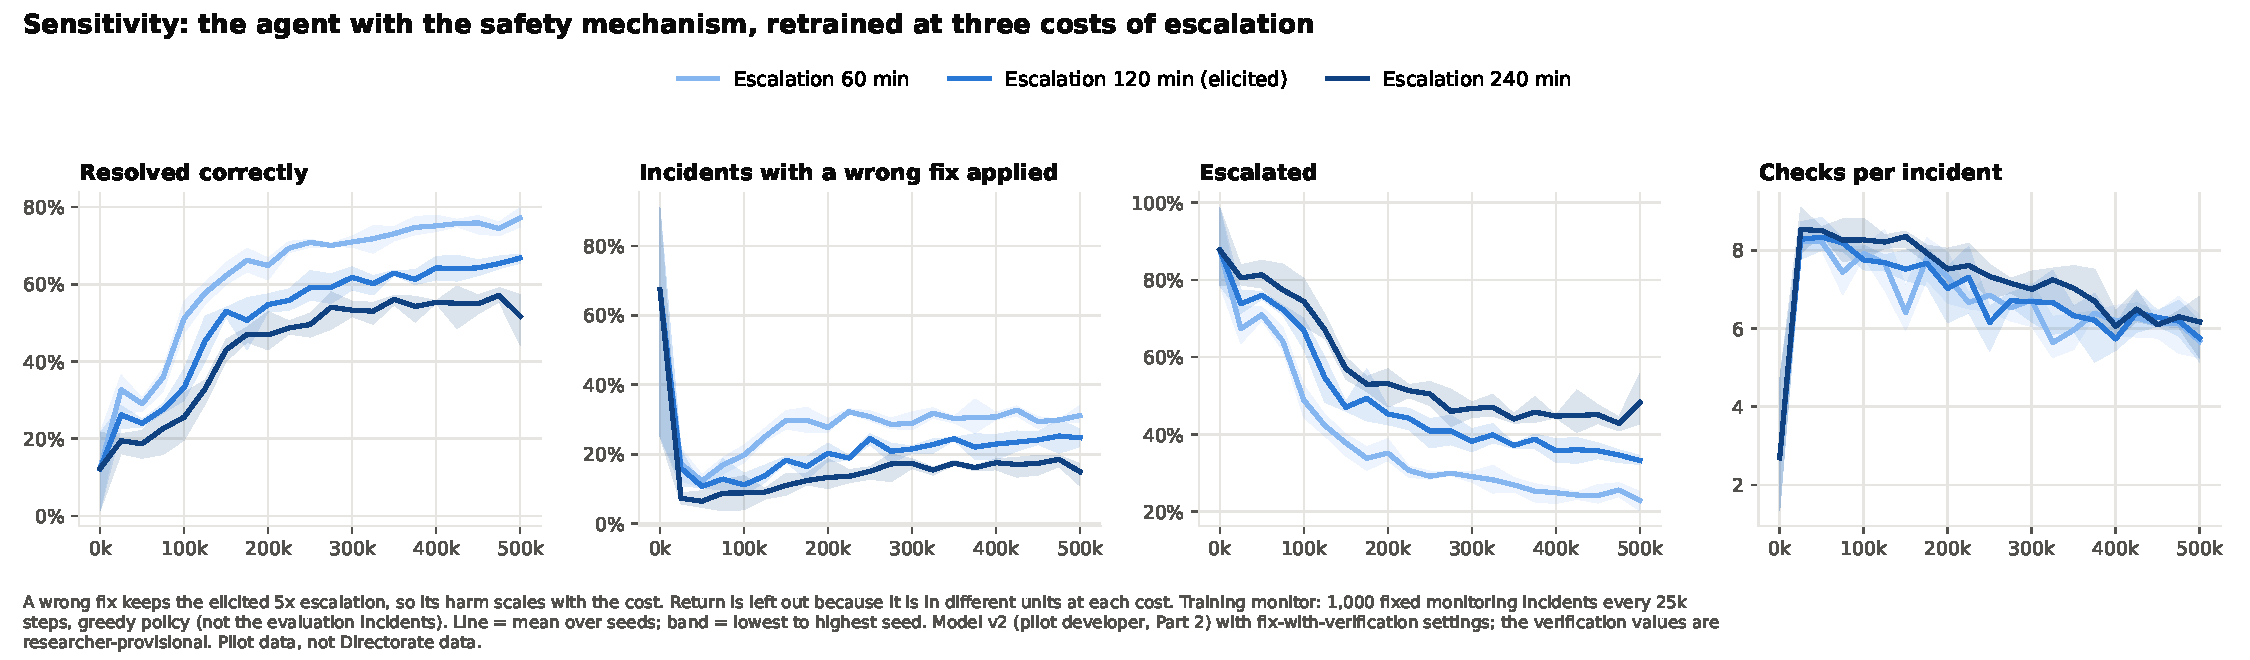
\includegraphics[width=\linewidth]{v3_training_sensitivity.pdf}
\caption{Training the agent with the safety mechanism at three escalation costs.}
\label{fig:train-sensitivity}
\end{figure}

\begin{table}[H]
\centering\small
\caption{Agent with the safety mechanism against the re-tuned threshold policy at three escalation costs (returns in hours).}
\label{tab:sensitivity}
\begin{tabularx}{\linewidth}{@{}lcccL@{}}
\toprule
Escalation & Threshold & Agent return & Threshold return & Agent minus threshold, per seed \\
\midrule
60 min & 0.55 & $0.92$ $[0.87, 0.96]$ & $1.08$ & $-0.21$, $-0.16$, $-0.12$ (all below zero) \\
120 min & 0.65 & $-0.41$ $[-0.50, -0.27]$ & $-0.38$ & $+0.11$, $-0.12$, $-0.09$ (level) \\
240 min & 0.80 & $-3.19$ $[-3.49, -2.98]$ & $-2.64$ & $-0.85$, $-0.46$, $-0.34$ (all below zero) \\
\bottomrule
\end{tabularx}
\end{table}

\begin{enumerate}[resume]
  \item \textbf{Behaviour moves in the expected direction.} As escalation and mistakes become costlier, the agent fixes less, escalates more (22\%, 32\%, 48\%) and applies fewer wrong fixes (31\%, 23\%, 15\%), as does the re-tuned threshold policy.
  \item \textbf{The conclusion about the threshold policy depends on the cost.} The agent is level with the threshold policy only at the elicited 120 minutes, and below it at both other costs. At 240 minutes, 12\% of its incidents end in forced escalations or the step limit, again because it proposes before it checks. Against the scripted, initial-symptom and always-escalate baselines its return is higher at every cost.
\end{enumerate}

% ---------------------------------------------------------------- 6
\section{Hypotheses, against the Chapter 3 criteria}\label{sec:hypotheses}

These are pilot readings with three seeds, not tests of the hypotheses.

\begin{table}[H]
\centering\small
\caption{Pilot readings of the hypotheses.}
\label{tab:hypotheses}
\begin{tabularx}{\linewidth}{@{}>{\raggedright\arraybackslash}p{3.2cm}>{\raggedright\arraybackslash}p{2.7cm}>{\raggedright\arraybackslash}p{3.4cm}L@{}}
\toprule
Hypothesis & Criterion (Chapter~3) & Pilot result & Reading \\
\midrule
\textbf{H1}: higher resolution accuracy than the initial-symptom, scripted and always-escalate policies, with no more investigation cost than the scripted checklist
 & At least 0.05 higher, intervals not overlapping
 & 67.6\% against 41.3\% (initial-symptom), 0\% (always escalate) and \textbf{88.3\% (scripted)}; 5.7 checks against 9
 & \textbf{Not supported}, because of the scripted checklist. On return the agent is far ahead ($-0.41$ against $-1.38$). Verification lets a fix-everything checklist resolve many incidents at a high cost, so resolution accuracy alone is a weak criterion in the fix-and-verify setting \\
\addlinespace
\textbf{H2}: higher compliant success than the unconstrained and penalty-only agents
 & At least 0.05 higher, intervals not overlapping
 & 67.6\% against 67.9\% (unconstrained) and \textbf{74.7\% (penalty-only)}
 & \textbf{Not supported.} The penalty-only agent learned the rules and broke none on these incidents \\
\addlinespace
Zero executed violations with the mechanism
 & Must hold on every incident
 & 0 of 15,000 agent incidents
 & \textbf{Holds} (verification of the implementation) \\
\addlinespace
Blocked proposals fall over training
 & Expected in Chapter~4
 & 35\% early, about 20 to 25\% at the end
 & \textbf{Only partly.} A block costs only a step in the pilot \\
\addlinespace
H3 (ambiguity) & Experiment 4 & Not run in this pilot & \\
\bottomrule
\end{tabularx}
\end{table}

\paragraph{What this means for the design.} The H2 result does not show that the safety mechanism is unnecessary. The penalty-only agent was evaluated only at the level it was trained on. In Phase~5 it broke rules in 4 to 7\% of incidents once checks started to go missing, while the mechanism stayed at zero. Experiment~4 is where that difference shows. Two changes follow from the pilot:
\begin{itemize}
  \item \textbf{Charge a block} (Chapter~3's $\lambda_{\text{block}}$, which the pilot set to zero), so that the agent learns to check before proposing. Report it as a design ablation. This needs the supervisor's agreement.
  \item \textbf{Judge H1 on return as well as resolution accuracy,} or state the criterion against the scripted checklist with verification in mind, since a policy that tries fix after fix can resolve a lot at a high cost.
\end{itemize}

% ---------------------------------------------------------------- 7
\section{The prototype}\label{sec:prototype}

The prototype puts the trained agent between a ticket and the action taken on it. It is shown in \file{dashboard/prototype\_app.py}: triage a ticket, all example cases, the outbox and draft pull requests, and the reader's error rates. The agent is \file{v3\_shielded\_seed0}, chosen on its training-monitor return, not on the evaluation incidents.

\paragraph{Verification in the prototype.} A fix for a code fault is applied to a staging copy of the fictional repository. It counts as working only if the incident's own reproduction test passes and no other test breaks. Any other fix is confirmed by the operator, or, for the example cases only, by the cause the case was written to show. A pull request is opened, as a draft, only after the fix is verified. Nothing is merged and nothing is sent; messages go to an outbox folder.

\begin{table}[H]
\centering\small
\caption{The eight example cases in the prototype.}
\label{tab:prototype}
\begin{tabularx}{\linewidth}{@{}>{\ttfamily\small}l>{\raggedright\arraybackslash}p{1.9cm}L>{\raggedright\arraybackslash}p{3.4cm}@{}}
\toprule
\normalfont Case & Written to show & Decision (v3 agent) & Earlier v2 agent (Phase 8) \\
\midrule
results\_approval & C02 & Fix C02, verified & Fix C02 \\
sign\_in & C08 & Fix C08, verified (staging test), no checks & Fix C08 \\
transcript\_duplicates & C07 & Fix C07, verified & Fix C07 \\
class\_results\_slow & C04 & Fix C04, verified (staging test) & Fix C04 \\
profile\_cache & C05 & Fix C05, verified (staging test) & Escalate \\
fees\_release & C06 & Escalate & Fix C07 (wrong) \\
payment\_gateway & C01 & Escalate at the step limit, 6 blocked proposals & Escalate \\
vague\_slow & none (escalate) & Tried C04, the fix failed, escalated & Fix C04 (wrong) \\
\bottomrule
\end{tabularx}
\end{table}

Six of eight cases end as intended, against four with the v2 agent. \texttt{vague\_slow} shows what verification adds: the agent's guess is caught by verification, not shipped. These eight cases were written by the researcher, as were the reader's keywords, so they show that the pipeline works, not how accurate it is. The pilot developer's 20 sample tickets measure accuracy. They are kept out of the repository because some may name real endpoints.

% ---------------------------------------------------------------- 8
\section{Discussion}\label{sec:discussion}

This section interprets the pilot results. It first discusses what they show and why, and then reads them against the five research questions and the three hypotheses of the study. Because the scenario model comes from one developer, uses three seeds and leaves several settings to the researcher (Section~\ref{sec:limits}), the discussion is about whether the method behaves as the study expects and where the design needs attention. It does not claim answers that only the main study can give.

\subsection{What the results show}

\paragraph{The agent learns the three-way decision.} Every agent starts at about $-10$~hours and ends between $-0.5$ and $-0.9$ on the monitoring incidents (Figure~\ref{fig:train-agents}). On the evaluation incidents it investigates (5 to 6 checks), fixes (two thirds to three quarters of incidents resolved) and escalates (about a quarter to a third). None of the three choices collapses into the others. The agent does not escalate everything, which costs 2~hours per incident, and it does not guess from the first symptom, which leads to a wrong fix in 29\% of incidents. This was the first thing the pilot had to show, because the rest of the study depends on it.

\paragraph{It reaches the threshold policy but does not beat it, and should not be expected to.} The threshold policy is given the likelihood model and computes the posterior probability of each cause exactly. The agent has to learn the same mapping from rewards alone. Reaching it within the seed intervals (Table~\ref{tab:paired}) is therefore a good result for a learner, not a failure. The agent's remaining gap shows in investigation: it runs about one check more than the threshold policy (5.7 against 4.7) and is still cutting checks at the end of training. The cost of those extra checks, not worse final decisions, is most of the gap in return. Longer training, or a block cost (below), is the likely remedy. In Phase~5, where the exact optimum could still be computed, the agents were about 0.65~h below it. With verification there is no exact reference, so this distance is unknown for the current setting.

\paragraph{Verification changes what ``good'' means.} Once a wrong fix is caught and the agent may try again, a policy can buy resolutions with repeated fixes. The scripted checklist does exactly that: nine checks, then the most probable fix, then the next. It resolves 88\% of incidents, the most of any policy, but applies a wrong fix in 30\% of them and spends nine checks every time, so its return ($-1.38$~h) is a full hour worse than the agent's ($-0.41$~h). The agent uses retries sparingly (7 to 12\% of incidents are resolved after a failed fix) and prefers to escalate when its evidence is weak. In the study's own terms, it trades a little resolution accuracy for far fewer wrong fixes and far less investigation. Resolution accuracy alone rewards the opposite trade, and this is why H1 is not supported (Section~\ref{sec:disc-hyp}).

\paragraph{The safety mechanism guarantees compliance but does not teach it.} The mechanism kept executed violations at zero on all 15,000 agent incidents, as it must. The unconstrained agent, which proposes a forbidden fix only about 1\% of the time, still broke a rule in 7.6\% of incidents, so even rare violations add up when nothing stops them. The cost of the mechanism shows in how the agent behind it behaves. About 22\% of its proposals are blocked, and that share settles near 20 to 25\% instead of falling to zero (Figure~\ref{fig:train-compliance}). Because a block costs only the step it uses, proposing a forbidden fix is a cheap way for the agent to find out which check the rule requires. The mechanism then sends the proposal back, and in 4\% of incidents a second block forces an escalation. This is the behaviour Chapter~3 set out to measure, and the pilot shows clearly that it depends on $\lambda_{\text{block}}$, which the pilot set to zero.

\paragraph{The penalty-only agent did best on compliance, but only where it was trained.} A penalty of 10 per rule-breaking action taught the penalty-only agent to stop proposing violations within 25k steps, and at the training level it broke no rule and had the highest compliant success (74.7\%). A penalty teaches; a mechanism enforces. The two differ when conditions change. In Phase~5, the penalty-only agent broke rules in 4.3\% of incidents at 20\% missing checks and 7.3\% at 40\%, conditions it had not seen in training, while the mechanism stayed at zero (Table~\ref{tab:sweep}). A deployed triage agent will meet conditions it was not trained on, so the guarantee matters more than the base-level comparison suggests.

\paragraph{Behaviour follows the cost of escalation in the right direction.} When escalation and mistakes become costlier, the agent fixes less and escalates more (22\%, 32\%, 48\% at 60, 120 and 240 minutes) and applies fewer wrong fixes (31\%, 23\%, 15\%), as the re-tuned threshold policy does. The reward design therefore steers the agent as intended. Its position relative to the threshold policy, however, holds only at the elicited 120 minutes, and at 240 minutes forced escalations rise to 12\%. A conclusion that the agent ``matches'' the strongest baseline is therefore sensitive to the cost of escalation, which is why the Directorate's estimate of that cost matters.

\paragraph{The prototype shows the decision layer working on text.} Six of the eight example cases end as intended, against four with the earlier agent, and the case written to be ambiguous (\texttt{vague\_slow}) shows the value of verification: the agent's wrong guess failed on staging and was escalated instead of shipped. In the prototype the language model only reads the ticket and logs into a fixed evidence form; the trained agent decides and the rule checker stays independent. This separation is the study's answer to the Directorate's question of how the approach differs from passing logs to an AI coding agent. The cases were written by the researcher, so they show that the pipeline works, not how accurate the reader is.

\subsection{The results against the research questions}\label{sec:disc-rq}

\begin{table}[H]
\centering\small
\caption{What the pilot contributes to each research question (Chapter~1).}
\label{tab:rq}
\begin{tabularx}{\linewidth}{@{}>{\raggedright\arraybackslash}p{4.6cm}>{\raggedright\arraybackslash}p{2.3cm}L@{}}
\toprule
Research question & Pilot evidence & What the pilot shows \\
\midrule
\textbf{RQ1.} How can ambiguous triage scenarios be represented in a controlled environment? & Scenario model v2, environment, Phases 1 to 3 gates & A practitioner could fill the workbooks, and the ratings became a working environment with separate controls for noise, missing checks and overlap. Partly answered: review by Directorate staff is still to come. \\
\addlinespace
\textbf{RQ2.} How can RL support decisions to gather information, apply permitted fixes and escalate? & Training curves; Table~\ref{tab:main}; prototype & A masked Double DQN learns all three choices at sensible rates and reaches the threshold policy. The contribution of each option (Experiment~3) was not tested. \\
\addlinespace
\textbf{RQ3.} How effectively can a rule-based safety mechanism prevent rule-breaking actions? & Experiment~2; Phase~5 sweep & Fully effective at preventing them (zero executed violations), but the agent behind it keeps relying on it while a block is free. \\
\addlinespace
\textbf{RQ4.} How does the approach compare with baseline policies? & Experiment~1; sensitivity analysis & Far ahead of the always-escalate, initial-symptom and scripted policies on return at every escalation cost; level with the threshold policy at 120 minutes, below it at 60 and 240. \\
\addlinespace
\textbf{RQ5.} How robust is the approach as evidence becomes incomplete, conflicting or ambiguous? & Phase~5 sweep only (earlier model, no verification) & Indicative only: the agent escalates more as checks go missing, and does not check more as noise rises. Experiment~4 was not run. \\
\bottomrule
\end{tabularx}
\end{table}

\paragraph{RQ1: representation.} The pilot shows that the representation planned in Chapter~3 can be built from a practitioner's judgement. One developer rated cause--check likelihoods on the verbal scale, named owners and rules, and later added the delegated check D11 and the code-fault flags in a second workbook. That was enough to produce an environment whose incidents the agents could learn from and whose behaviour passed the Phase~1 to~3 gates. Two lessons carry over to the main elicitation. First, the fix-and-verify variant needs values the workbooks did not ask for (remedy times, harms and the number of retries), which the researcher set here and which need a third workbook. Second, the reward values were not all elicited. The correct-fix reward and the check costs are the researcher's, and Section~\ref{sec:results} shows that the conclusions move with the escalation cost. RQ1 is therefore answered in part. The representation works, but it is not yet validated by the Directorate.

\paragraph{RQ2: the role of reinforcement learning.} The agent learns when to look further, when to act and when to hand over, without being told the likelihood model, and ends level with a policy that is given it. That is the core claim behind RQ2, and the pilot supports it. What the pilot does not yet show is why the three-way choice is needed. Experiment~3, which removes the option to investigate or to escalate, was not run. The pilot also shows a weakness of the learned policy: it investigates more than necessary and keeps proposing actions before running the checks the rules require. Both are matters of training and reward design rather than of the method itself.

\paragraph{RQ3: the safety mechanism.} On the question as asked, the pilot answer is clear: the mechanism prevented every rule-breaking action, at the base level and at every level of the Phase~5 sweep, while the unconstrained agent broke rules in 6 to 13\% of incidents and the penalty-only agent in up to 7\% once checks went missing. The pilot adds a second finding that the question does not ask for but the thesis should report. An agent that is stopped for free learns to lean on being stopped. Of the two studies in the systematic review that measured a hard rule mechanism, neither reported how blocked proposals change over training. The pilot shows that this rate is the measure that reveals the problem, and that the cost of a block is the parameter that controls it.

\paragraph{RQ4: comparison with baselines.} The answer depends on which measure is used. On return, the measure the agent optimises, it is far ahead of the always-escalate, initial-symptom and scripted policies at every escalation cost, and level with the threshold policy at the elicited cost. On resolution accuracy, the scripted checklist is ahead because verification lets it keep trying. On escalation quality the learned agents and the threshold policy are close (MCC 0.54 to 0.57). Chapter~3 already requires that return is never reported alone. The pilot suggests the converse for the fix-and-verify setting: resolution accuracy should not be read alone either, but together with the wrong-fix rate and the investigation cost.

\paragraph{RQ5: robustness.} The fix-and-verify agents were evaluated only at the base level, so the pilot cannot answer RQ5. The Phase~5 sweep, run on the earlier model without verification, gives a first indication (Table~\ref{tab:sweep}). It is discussed with H3 below.

\subsection{The results against the hypotheses}\label{sec:disc-hyp}

\paragraph{H1: decision quality.} H1 states that the agent achieves higher decision quality than the baselines, and the decision criteria make this operational as higher resolution accuracy than the initial-symptom, scripted and always-escalate policies, with no higher investigation cost than the scripted checklist. The agent passes against two of the three (67.6\% against 41.3\% and 0\%) and on investigation cost (5.7 checks against 9), and fails against the scripted checklist (67.6\% against 88.3\%). H1 is therefore not supported in the pilot. The discussion above suggests that this says more about the criterion than about the agent. In the setting without verification (Phase~5) the scripted checklist resolved 70.6\%, also ahead of the agents (51.5\% to 58.8\%), but with verification its lead grows because it can retry every wrong fix, while its return stays an hour behind. Two options are open for the main study, and both need the supervisor's agreement before the Directorate experiments, since the criteria were fixed in advance: keep the criterion and report H1 as not supported, with return and wrong-fix rate alongside; or judge decision quality on a measure that counts the cost of a wrong fix, such as return or resolution accuracy at a fixed wrong-fix rate. Changing the criterion after seeing results would not be acceptable, so this has to be settled now, on pilot data, if at all.

\paragraph{H2: compliant success with the mechanism.} H2 is not supported either. The agent with the mechanism (67.6\%) is level with the unconstrained agent (67.9\%) and below the penalty-only agent (74.7\%). Two things explain it. First, the unconstrained agent's violations were few, so removing them costs it little compliant success. Second, the mechanism's agent loses resolutions to forced escalations and to the extra escalation it learned while being blocked, which is the zero-block-cost effect again. The Phase~5 sweep adds a qualification: even at 40\% missing checks, where the penalty-only agent broke rules in 7.3\% of incidents, the mechanism's agent had lower compliant success (32.5\% against 41.9\%), because it escalated far more (56\% against 35\%). The mechanism protects against violations without improving compliant success in this pilot. If H2 is to be supported in the main study, the agent behind the mechanism must learn to check before proposing, which is what a block cost is designed to achieve. The pilot therefore turns $\lambda_{\text{block}}$ from a detail of the reward into a variable that decides H2, and it should be reported as an ablation.

\paragraph{H3: response to ambiguity.} H3 was not tested, because Experiment~4 was not run with the current agents and the overlap control was not swept. The Phase~5 sweep of the earlier agents, which recommended a fix without verification, gives the readings in Table~\ref{tab:sweep}. They use the criteria for H3a and H3b, but over the smaller pilot ranges (noise up to 0.2, missing checks up to 0.4) and with five seeds.

\begin{table}[H]
\centering\small
\caption{Phase~5 sweep, agent with the safety mechanism (earlier model v1, no verification; mean of five seeds; 2,000 incidents per level). Indicative readings for H3, not tests. The penalty-only agent's executed violations are shown for comparison.}
\label{tab:sweep}
\begin{tabular}{@{}lcccccc@{}}
\toprule
Level & Return (h) & Resolved & Escalated & Coverage & Checks & \shortstack{Penalty-only:\\rule broken} \\
\midrule
Noise 0, missing 0 & $0.32$ & 58.7\% & 27.1\% & 72.9\% & 4.75 & 0\% \\
Noise 0.1, missing 0 (base) & $-0.28$ & 51.5\% & 33.2\% & 66.8\% & 4.80 & 0\% \\
Noise 0.2, missing 0 & $-0.95$ & 44.4\% & 38.1\% & 61.9\% & 4.86 & 0\% \\
Noise 0.1, missing 0.2 & $-0.85$ & 41.7\% & 44.9\% & 55.1\% & 5.02 & 4.3\% \\
Noise 0.1, missing 0.4 & $-1.33$ & 32.5\% & 56.4\% & 43.6\% & 5.18 & 7.3\% \\
\bottomrule
\end{tabular}
\end{table}

\begin{itemize}
  \item \textbf{H3a (missing evidence):} the expected pattern. From the base level to 40\% missing checks, escalation rises from 33\% to 56\% and checks rise by only 0.4, below the 0.5 that counts as a difference. On the pilot range this reading is consistent with H3a.
  \item \textbf{H3b (unreliable evidence):} only half the expected pattern. Coverage falls as noise rises (66.8\% to 61.9\%), but the agent does not check more (4.80 to 4.86). It responds to noise by escalating, not by corroborating. A plausible reason is that the agent was trained at one noise level, so it never learned that extra checks pay off when results are less reliable. The randomised training of Chapter~3 is designed for this case.
  \item \textbf{H3c (overlapping evidence):} no evidence. The overlap control was not swept.
\end{itemize}

These readings come from the earlier model and must be repeated with the fix-and-verify agents. They suggest that robustness is where the main study will find its clearest result, both for H3 and for the difference between the mechanism and a penalty.

\subsection{Overall: the research question}

The study asks how an agent should decide, under ambiguous evidence, whether to investigate, fix or escalate an IT incident while respecting the organisation's rules, and whether reinforcement learning with an independent safety mechanism is a sound way to make that decision. On the pilot evidence the answer is a qualified yes. The approach works end to end, from a practitioner's ratings to a trained agent and a prototype acting on tickets and logs. The agent learns a sensible three-way policy, reaches the strongest baseline on return, responds to the cost of escalation and to missing evidence in the expected direction, and never executes a forbidden action when the mechanism is in place.

The pilot is just as clear about what does not yet hold. Neither formal hypothesis tested is supported. Each failure has an identifiable cause that can be addressed before the main study: a resolution-only criterion that rewards repeated fixes once fixes are verified, and a zero block cost that lets the agent rely on the mechanism instead of learning the rules. The pilot thus does what a pilot should. It confirms that the method is workable, shows that the outcome of the hypotheses depends on two design choices that would otherwise have gone unexamined, and gives the Directorate elicitation a concrete list of values to ask for. The decisions it leaves are the supervisor's: whether to charge a block, and how H1 should be judged in the fix-and-verify setting.

% ---------------------------------------------------------------- 9
\section{Limits}\label{sec:limits}

\begin{itemize}
  \item \textbf{One developer, not the Directorate.} The model, the costs and the rules come from one person. The pilot's purpose is to test the method.
  \item \textbf{Researcher-set values.} The correct-fix reward, check costs, the verification settings (apply times, harm weights, two-fix limit) and the penalty of 10 are the researcher's. The verification settings in particular go to the developer in a Part~3 workbook.
  \item \textbf{Three seeds.} Chapter~3 plans ten. Several differences in Section~\ref{sec:results} sit inside the seed intervals.
  \item \textbf{Block cost of zero.} This differs from Chapter~3 and probably explains most of the safety mechanism's cost here.
  \item \textbf{Base ambiguity level only.} Missing checks, more noise and overlap (Experiment~4) and the action ablations (Experiment~3) were not run.
  \item \textbf{Reliable verification.} A fix that clears the symptoms is assumed to have removed the true cause.
  \item \textbf{No exact reference.} The exact solver does not model verification, so the agents' distance from the best possible return is unknown in this setting (it was 0.65~h in Phase~5, without verification).
\end{itemize}

% ---------------------------------------------------------------- 9
\section{Next steps}

\begin{enumerate}
  \item Take the results and the questions in the pilot plan (Section~5) to the Directorate; ask for a Part~3 workbook on remedy times and harms.
  \item Agree the block penalty with the supervisor; run it as an ablation of the agent with the safety mechanism.
  \item Revisit the H1 criterion for the fix-and-verify setting.
  \item Experiment~4 on the saved agents (missing checks and noise), where the penalty-only agent is expected to break rules and the mechanism is not.
  \item Score the reader on the developer's 20 sample tickets (keyword and, with an API key, the Claude reader).
\end{enumerate}

\section*{Reproduce}

\begin{small}
\begin{verbatim}
python -m experiments.pilot.run_comparison train --parallel 5      :: 15 runs, about 3.5 h
python -m experiments.pilot.run_comparison evaluate                :: about 17 min
python -m experiments.pilot.plot_v3_training                       :: training figures
python -m experiments.pilot.evaluate_prototype --out prototype_v3  :: the eight cases
streamlit run dashboard/prototype_app.py                           :: the prototype
\end{verbatim}
\end{small}

\end{document}
